\chapter{\label{chap:evaluation}Evaluation}

% This chapter reports the offline gates and the supervised Six-layer live
% evaluation. Live results must be written only from the secret-free evidence
% records produced by the approved protocol.
% SOURCE: docs/research/evaluation/small-scenario-matrix.json
% SOURCE: docs/research/evaluation/live-evaluation-protocol.md
% TARGET: ~12–18 pages

\section{Experimental Setup}
\label{sec:eval-setup}
The evaluation separates deterministic offline checks from supervised provider
execution. Its live Core matrix contains three provider-local cases and the six
directed pairs between AWS, Azure, and GCP. Each successful Core observation
sends ten identifiable ingress messages and requires the ten expected values
at authenticated destination hot-storage readback. The unit of comparison is
this bounded contract, not an entire provider product or a production workload.

Higher responsibilities were evaluated separately: local command return on all
three providers, Event-to-L4 projection on AWS and Azure, and graphical L3-to-L5
reads on AWS and Azure. GCP L4/L5 were excluded as an explicit implementation
scope finding. Successful adjacent cuts are not treated as proof of their
composition through the application. The research questions are unchanged.

\section{E2E Test Framework}
\label{sec:eval-framework}
Before a live attempt, the procedure checks identity, graph-derived readiness,
artifact and configuration references, resource scope, execution bounds, and
cleanup ownership. Apply, verification, Destroy, and independent residual
inventory are recorded separately. Failed attempts are preserved rather than
replaced by the successful retry. Credentials and raw operational records remain
private; the repository publishes secret-free result summaries and limitations.

Phase durations and resource lifecycle observations measure different things.
Main Apply excludes preceding image publication and, where applicable, a
separate Kubernetes stage. Verification includes sending and polling. Terraform
Destroy excludes independent inventory and any separately recorded Kubernetes
removal. These columns therefore cannot simply be summed into total lifecycle
time. Individual resource creation records are also not counts of unique
services when retries or multiple phases are present.

\section{Scenario Coverage}
\label{sec:eval-scenarios}
All nine Core paths passed their ten-message assertion. This establishes the
tested telemetry transport, processing, Eventing, and hot-storage path under
the recorded conditions. It does not establish nine complete-profile passes,
directed command return, cross-cloud Twin projection, storage-tier transitions,
or exhaustive allocation coverage. A representative application workflow is a
separate completion check, not a reason to repeat all nine successful Core cases.

\section{Results}
\label{sec:eval-results}
Table~\ref{tab:core-observations} reports one successful observation per path.
Durations are seconds, rounded to one decimal. The detailed execution record
retains revisions, failures, resource timings, and differing readiness
conditions.\footnote{Repository evidence summaries:
\texttt{docs/research/evaluation/core-telemetry-results.md} and
\texttt{docs/plans/2026-09-16\_poc\_core\_evaluation.md}.}

\begin{table}[htbp]
\centering
\small
\caption{Successful Core observations; all rows verified ten of ten messages.}
\label{tab:core-observations}
\begin{tabular}{@{}lrrrr@{}}
\toprule
Path & Main Apply & K8s Apply & Verification & TF Destroy \\
\midrule
AWS $\rightarrow$ AWS & 98.8 & -- & 56.0 & 71.8 \\
Azure $\rightarrow$ Azure & 668.8 & -- & 209.2 & 782.6 \\
GCP $\rightarrow$ GCP & 791.5 & 139.0 & 19.0 & 542.9 \\
Azure $\rightarrow$ AWS & 541.5 & -- & 32.9 & 228.8 \\
AWS $\rightarrow$ Azure & 668.2 & -- & 148.6 & 889.3 \\
AWS $\rightarrow$ GCP & 604.9 & -- & 26.6 & 443.3 \\
Azure $\rightarrow$ GCP & 941.7 & -- & 48.3 & 479.3 \\
GCP $\rightarrow$ AWS & 471.4 & 136.9 & 19.5 & 561.7 \\
GCP $\rightarrow$ Azure & 654.1 & 116.6 & 220.3 & 948.4 \\
\bottomrule
\end{tabular}
\end{table}

These observations are not repeated benchmark trials. In particular, Azure's
local case used the documented warm HTTP condition; provider readiness and
cold-start conditions were not identical across rows. The older AWS local case
has no individual message-to-persistence samples. Missing measurements are not
reconstructed from verification duration or presented as zero.

Separate local simulator-command observations recorded one correlated return
and exact L3 readback per provider: 13.646645 seconds on AWS, 38.264408 seconds
on Azure, and 28.965664 seconds on GCP. These single samples demonstrate the
bounded command contract, not latency distributions or provider rankings.
Deployed Event-to-L4 consumers subsequently passed on AWS and Azure.

The separate graphical L5 checks rendered three exact seeded raw points and
three hourly records in two panels on both providers. Unauthenticated access
was rejected (AWS HTTP 403, Azure HTTP 401). Deployment, verification, and
Destroy took 40.512/2.104/15.376 seconds on AWS and
561.910/7.190/711.249 seconds on Azure. These are seeded L3-to-L5 observations,
not simulator-to-L5 evidence or Managed Grafana equivalence.\footnote{The
scoped L5 record is \texttt{docs/plans/2026-10-05\_minimal\_l5\_evidence.md}.}

The successful cuts were destroyed and independently checked for active
run-owned residuals. Inactive provider deletion markers are reported separately.
A later AWS reconciliation found its command markers absent; the recorded GCP
deleted identity/Logging markers are not active resources. These dated checks
are not a current global account inventory.

Provider billing, planning allowances, and modeled monthly allocations are
distinct quantities. Account or subscription totals cannot be attributed to
one run without reconciliation; failed attempts, image publication, and cleanup
also contribute to the cost of obtaining evidence. No paired live Five-layer
comparison or isolated causal Event-Layer cost saving is established by the
successful functional cuts.

\subsection{Frozen cost comparison and scale sensitivity}
The existing Optimizer was rerun offline with the eight planned complete-profile
placements and the immutable Small, Medium, and Large inputs. All calculations
use the same reviewed baseline pricing snapshots fetched on August 25, 2026.
The result records workload, pricing, candidate, and plan digests and reproduces
byte-identically. No live capacity or cost observation is implied.

\begin{table}[htbp]
\centering
\small
\caption{Modeled monthly USD; focal-edge labels denote the fixed matrix placements.}
\label{tab:modeled-costs}
\begin{tabular}{@{}lrrr@{}}
\toprule
Placement & Small & Medium & Large \\
\midrule
AWS local & 126.84 & 3,448.38 & 117,627.25 \\
Azure local & 142.25 & 7,850.49 & 135,864.88 \\
AWS $\rightarrow$ Azure & 145.69 & 7,983.96 & 150,345.32 \\
Azure $\rightarrow$ AWS & 147.05 & 8,049.70 & 137,229.15 \\
AWS $\rightarrow$ GCP & 100.54 & 3,663.18 & 126,606.25 \\
GCP $\rightarrow$ AWS & 282.27 & 11,575.34 & excluded \\
Azure $\rightarrow$ GCP & 213.84 & 6,192.29 & 131,680.41 \\
GCP $\rightarrow$ Azure & 224.34 & 7,602.59 & excluded \\
\bottomrule
\end{tabular}
\end{table}

The lowest Small cost among these eight placements is AWS with GCP Eventing
and all other components on AWS: 26.30 USD/month (20.73\%) below AWS local,
the cheaper admissible local baseline. AWS local becomes cheapest among this
set for Medium and Large. These are discrete workload-scale comparisons:
multiple inputs change together. They are not an isolated parameter effect,
proof of the global minimum, or Medium/Large live qualification. The two Large
GCP-ingress placements fail the existing admissibility gate; missing costs are
not zeros. A complete GCP-local profile remains excluded by L4/L5 scope.

Small AWS local assigns 105.173677027 USD/month to Eventing, principally
Kinesis (105.171471123). A remote placement also changes source/bridge and
transfer charges outside this component subtotal. Total candidate costs, not
the difference between broker prices alone, determine the comparison.
The reproducible ledger and its limitations are published in
\texttt{docs/research/evaluation/poc-cost-model-results.json} and the
accompanying method note. The historical component-level Eventing decision
calculator reproduces separately under its original assumptions; it is not
substituted for the current complete-profile calculation.

\section{Deployment Challenges Discovered}
\label{sec:eval-bugs}
The normal application check exposed defects not covered by the isolated
provider cuts: a browser-sensitive authenticated redirect, confusion between
uploaded source inventory and restored runtime metadata, an invalid Terraform
state-inspection argument, and attachment of the resolved graph after rather
than before credential validation. These are operationalization findings for
RQ1, not changes to the logical architecture. Separate regression tests and
commits preserve the corrections; their local success does not itself establish
a live application pass.

One normal AWS application deployment subsequently succeeded at runtime revision
\texttt{cd4e7b39} in 270.536770 seconds, including image foundation/publication
and SDK postapply. The UI reconnect retained the same single operation. The
downloaded simulator first delivered value 42 and a correlated command in
30.394552 seconds, but its L4 assertion failed because the test input omitted
the contract's explicit projection-candidate marker. That observation remains
failed for the combined assertion, not rewritten as success.

A second marked sample in the same deployment passed exact L3 raw/hourly
readback, deployed Event-to-L4 value/sequence/timestamp, and both graphical L5
panels; its command receipt took 2.389944 seconds and combined verification
9.381697 seconds. No seeded record or direct Twin update supplied this result.
The normal L5 action fetched HTTP 200; browser automation did not expose its
separate blob popup, so visual inspection rendered an unchanged saved copy of
the returned HTML. Universal popup behavior is not claimed.

\begin{figure}[htbp]
\centering
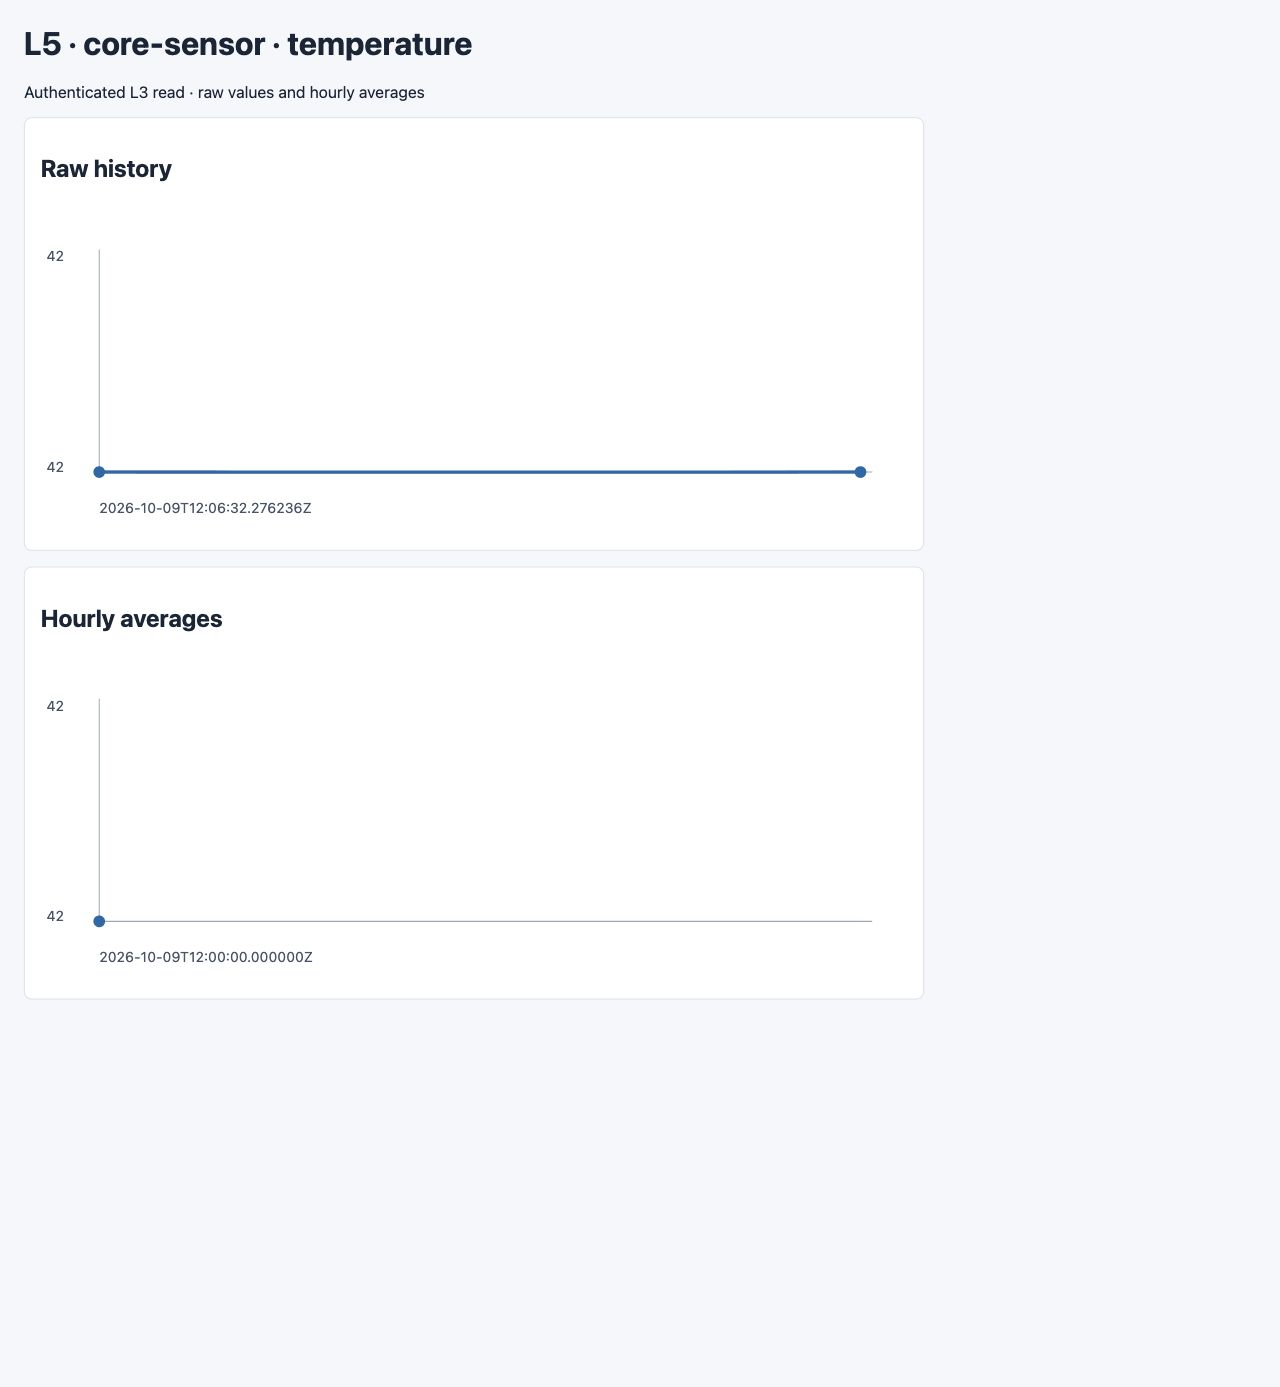
\includegraphics[width=0.68\textwidth]{application-l5-2026-10-09.jpg}
\caption{Actual L5 snapshot: two simulator raw points and their hourly average,
both with value 42. Rendering uses the unchanged authenticated HTML response.}
\label{fig:application-l5}
\end{figure}

Journaled cleanup removed the exact SDK-owned simulator certificate, policy and
Thing before normal Destroy. The first strict Destroy failed after fallback
(157.246469 seconds); a second reconciled stale state and succeeded
(30.976129 seconds). Independent scans found zero active residuals in both the
successful and earlier failed namespaces, with one inactive IoT marker in each.
The old namespace retains its tombstone-related state entry. The application
record retains five earlier failed Deploy attempts and 110 creation-completion
observations for the successful run. This is a scoped composed observation with
explicit cleanup and UI conditions, not nine complete-profile passes.
\footnote{\texttt{docs/research/evaluation/application-closeout-results.md}.}

\section{Threats to Validity}
\label{sec:eval-validity}
Internal validity is limited by implementation corrections between attempts,
provider transients, cold starts, and cross-provider clock alignment. External
validity is limited by one supervised environment, curated Small inputs, fixed
regions, and no concurrent or long-running trials. Construct validity is
limited by the selected contracts and reduced L5 responsibility. The evaluation
supports named functional observations and a traceable method; it does not
support statistical performance rankings, exhaustive equivalence, or causal
cost claims from unmatched successful runs.
